\documentclass[10pt]{article}
\usepackage[margin=0.72in]{geometry}
\usepackage{graphicx}
\usepackage{booktabs}
\usepackage{amsmath}
\usepackage{amssymb}
\usepackage{xcolor}
\usepackage{listings}
\usepackage[hidelinks]{hyperref}
\usepackage{float}
\usepackage{caption}
\captionsetup{font=small,labelfont=bf}
\lstset{basicstyle=\ttfamily\fontsize{5.8}{6.8}\selectfont,
        frame=single, rulecolor=\color{gray!55}, columns=fullflexible,
        aboveskip=2pt, belowskip=2pt, breaklines=true}
\title{\vspace{-1.2em}Learning to Write Graph Algorithms:\\A Harness Developing Agent from Examples to 100k-Node Graphs}
\author{CS 5624 project --- agent-generated draft for author rewrite}
\date{November 2026}

\begin{document}
\maketitle
\thispagestyle{empty}

\begin{abstract}
We study a Harness Developing Agent (HDA): an LLM that receives a few
input/output examples for a graph task and writes one self-contained C++17
program, which is then run on held-out graphs up to 100{,}000 nodes. The agent
develops only on 4--50-node graphs and is scored on strict graph sizes; a
program that is correct but slow passes validation and fails at scale. For ten
polynomial-time tasks, after fixing an ambiguous query encoding, nine tasks
reach validation accuracy 1.000 and eight score 100\% on every test split; max
flow is the clean small-to-large failure (100\% through 2{,}000 nodes, 30\% on
10k--20k). For three NP-hard tasks we replace exact-match scoring with pure
normalized quality under a feasibility gate. Max clique and maximum independent
set reach 0.93 and 0.97 of optimal on small exact references; min vertex cover
is the weak case (0.49, all feasible, never optimal). At scale, MIS quality
falls from 0.75 on 500--1000 nodes to 0.15 on 2{,}000 and 0.05 on 10k--20k,
while MVC becomes infeasible above small graphs. The pipeline, prompts, splits,
logs and scoring code are released with the paper.
\end{abstract}

\section{Introduction}
The usual graph-agent setup gives the model a Python sandbox with NetworkX.
That measures tool use, not algorithm development: the library supplies the
algorithm and the model only needs to call it. We instead ask the model to
write the harness itself. For one graph task it sees a short problem statement
(optionally hidden) and $k=5$ input/output examples, and must produce a single
C++17 program. The program is compiled, tested on the examples, and refined
through a compiler/test loop. Only small graphs are used for development; the
final program is evaluated on fresh graphs of increasing size.

Our contributions are:
\begin{itemize}\setlength\itemsep{1pt}
\item an HDA interface with a real compiler, per-example verdicts, a
  non-reusable code contract, and rolling context;
\item a diagnosis and fix of an ambiguous query encoding that made
  query-based tasks return $-1$ even with the statement given;
\item a phase-1 evaluation of ten polynomial-time tasks up to 100k nodes;
\item a phase-2 scoring rule for NP-hard tasks: pure normalized quality with
  a hard feasibility gate, exact references on small graphs and frozen
  best-known references above that.
\end{itemize}

\section{Methods}
\subsection{Setting and tasks}
Phase~1 has ten polynomial-time tasks: shortest path (weighted
$s$--$t$), reachability (directed), connected-component count, cycle detection,
diameter, common-neighbor count, triangle count, bipartite check, MST weight
and max flow. Answers are exact single tokens or node lists.

Phase~2 adds three NP-hard maximization/minimization tasks: maximum clique,
maximum independent set (MIS) and minimum vertex cover (MVC). The HDA prints a
node list, so the evaluator can check feasibility before scoring quality.

\subsection{Agent interface and compiler loop}
Figure~\ref{fig:loop} shows one run. The agent receives a system prompt, the
task statement in the \emph{given} condition (nothing in \emph{hidden}), five
inline examples, the previous validation feedback, the best program so far and
the current statement. Every reply contains a statement, optional reasoning,
one \texttt{cpp} block and one action tag.

The agent can call \texttt{compile} (diagnostics only), \texttt{test} (compile
and run every seen example), \texttt{run} (its own input) and \texttt{stress}
(a C++ generator for large inputs). Tool output is appended as the next user
message, so the model sees compiler errors and per-example verdicts and can
edit the program in a loop. A bare action without a complete \texttt{cpp} block
is rejected; older code is not silently reused. Generation stops at
\texttt{</action>}; old replies are dropped so the prompt does not grow.

\begin{figure}[H]
\centering
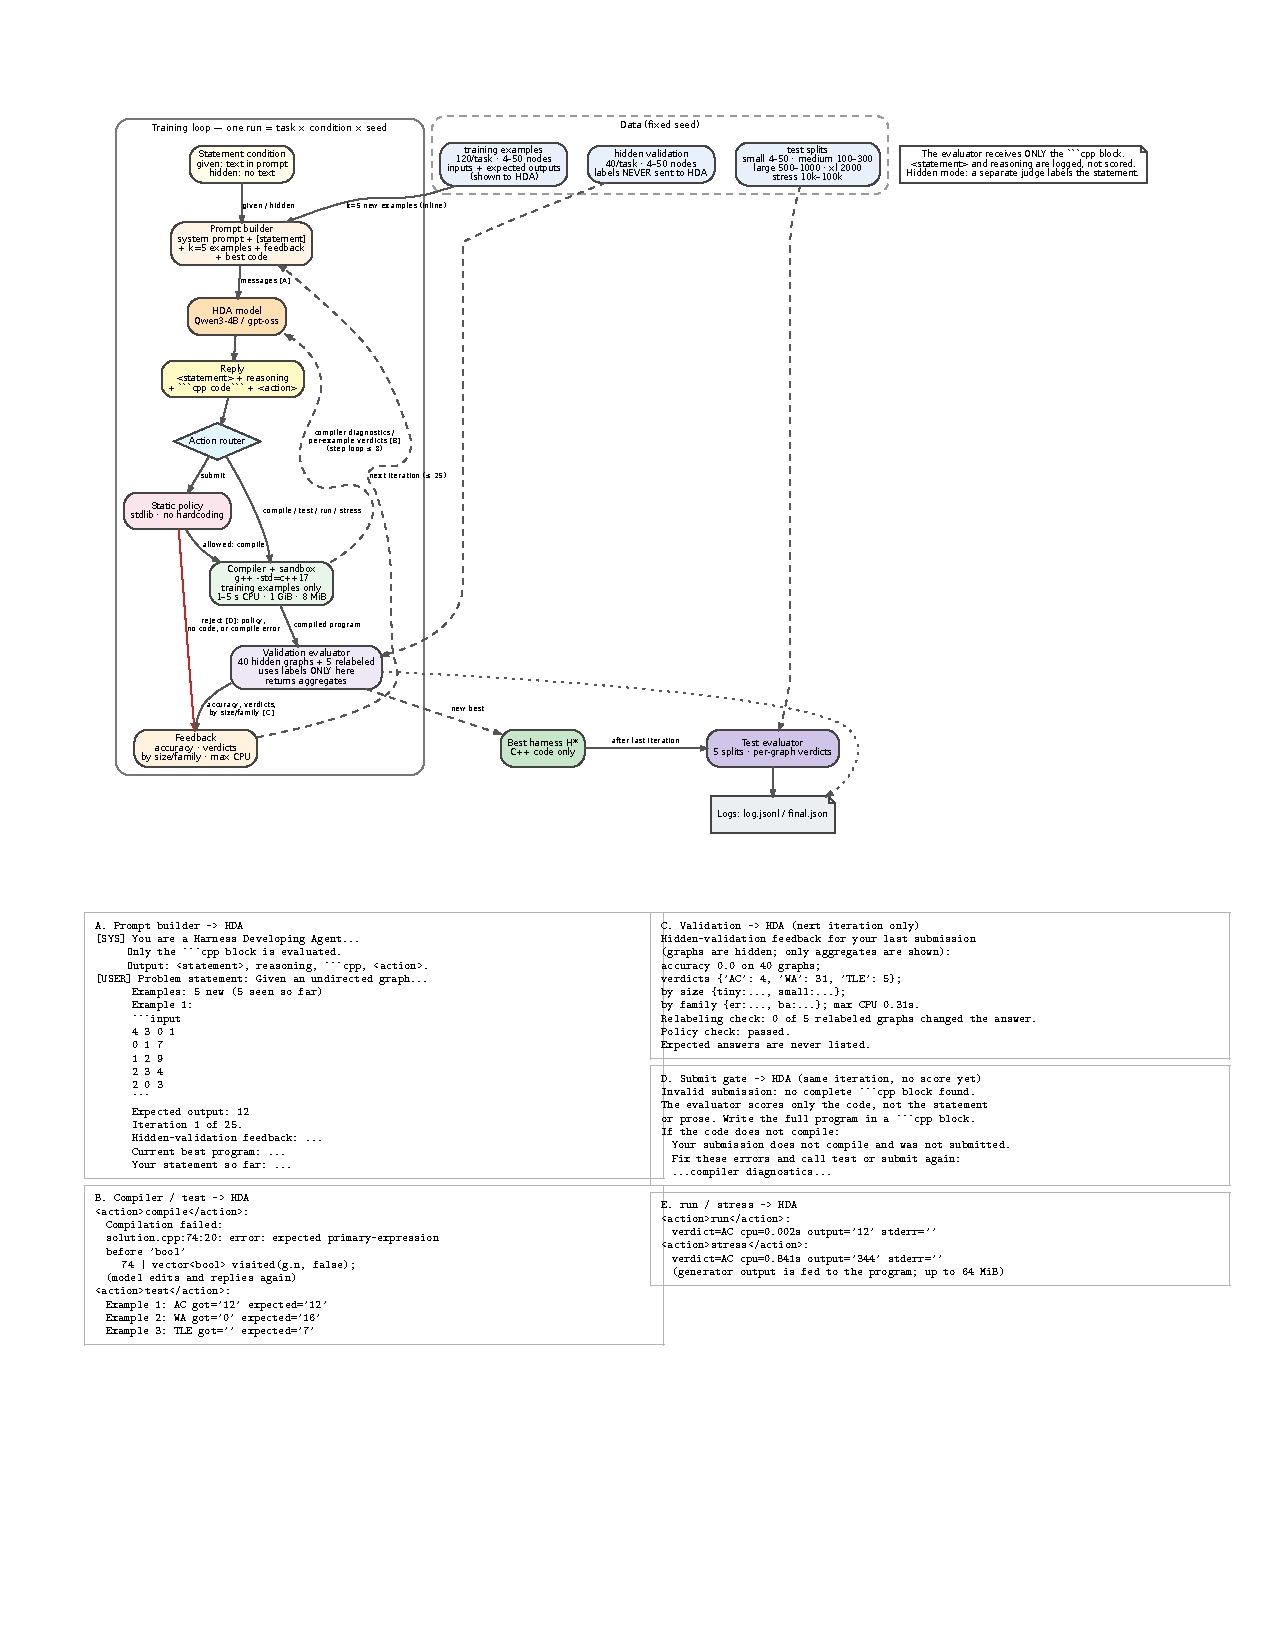
\includegraphics[width=0.64\linewidth]{figures/hda/hda_diagram_full.pdf}
\caption{Training/validation loop and the exact message structures A--E.
Only the \texttt{cpp} block is compiled and scored; validation labels never
reach the HDA.}
\label{fig:loop}
\end{figure}

\subsection{Input format and the query fix}
The last input line is \texttt{k q1 ... qk}. The first number is the
\emph{number of query arguments}, not a type code. The loader exposes
\texttt{query\_k} and \texttt{query[0..]}; for a $k=2$ task, \texttt{2 s t}
means \texttt{query\_k=2}, \texttt{query[0]=s}, \texttt{query[1]=t}. Before
this fix, the model searched for a type tag \texttt{2} inside \texttt{query}
(which held only \texttt{[s,t]}), left the endpoints unset, and returned
$-1$. The failed run was therefore an interface ambiguity, not a shortest-path
algorithm failure.

\subsection{Training loop and data}
For each task, condition and seed we run three iterations. Each iteration
draws five new examples, gives the model up to eight tool steps, submits the
latest program, applies a static policy check (standard library only, no file
I/O/threads/system calls, no hardcoded answer tables), compiles it, and scores
it on 40 hidden small-graph validation instances. Five validation graphs are
re-run with fresh node IDs; failures reduce the score. Feedback contains
accuracy or mean quality, verdict counts, size/family breakdowns, maximum CPU
and relabeling results. $H^*$ is the best-validation submission.

Phase-1 splits range from 4--50 nodes (\texttt{examples}, \texttt{val},
\texttt{test\_small}) to 100--300, 500--1000, 2{,}000 and 10k--100k. Phase-2
uses 4--50 for examples/validation and 100--300, 500--1000, 2{,}000 and
10k--20k for test. Node IDs are permuted and edge order is shuffled. Phase-1
ground truth is human-written C++ cross-checked against NetworkX; phase-2
small labels are exact NetworkX optima. Above 60 nodes the phase-2 reference
is a frozen multi-start heuristic (greedy degree/random orders, 16 starts for
clique and 20 for MIS/MVC). Thus $q=1$ in phase 2 means ``matched best known''
above 60 nodes, not ``proved optimal''.

\subsection{Scoring}
Phase~1 uses exact answer accuracy. Phase~2 uses \emph{pure normalized
quality} with a hard feasibility gate:
{\small
\[
q=\begin{cases}
0 & \text{infeasible, timeout, crash}\\
\operatorname{clip}(\text{value}/\text{reference},0,1) & \text{max clique, MIS}\\
\operatorname{clip}(\text{reference}/\text{value},0,1) & \text{MVC}
\end{cases}
\]}
A valid but poor heuristic receives partial credit in proportion to its
objective value; merely feasible solutions get no bonus. The metrics are mean
$q$, feasible rate, optimal rate (small exact graphs), verdict mix, maximum
CPU and breakdowns by size and family.

\section{Results}
\subsection{Phase 1: polynomial-time tasks}
After the query fix, the ten given-statement runs used $k=5$, three
iterations, 32k context, temperature 0.2 and a 4{,}096-token safety guard.
Nine tasks reach validation 1.000; diameter reaches 0.900. Table~\ref{tab:p1}
and Figure~\ref{fig:p1} show the test results. Eight tasks are perfect on all
five splits, triangle counting loses 3.3 points only on large, diameter ranges
from 70\% to 83.3\%, and max flow is 100\% through 2{,}000 nodes but only 30\%
on the 10k--20k stress split. The max-flow program is therefore correct but
does not scale, which is exactly the failure mode the benchmark is designed to
expose.

\begin{table}[H]
\centering
\small
\begin{tabular}{lrrrrrr}
\toprule
task & val & small & medium & large & xl & stress \\
\midrule
bipartite\_check & 100.0\% & 100.0\% & 100.0\% & 100.0\% & 100.0\% & 100.0\% \\
common\_neighbors & 100.0\% & 100.0\% & 100.0\% & 100.0\% & 100.0\% & 100.0\% \\
connected\_components & 100.0\% & 100.0\% & 100.0\% & 100.0\% & 100.0\% & 100.0\% \\
cycle\_detection & 100.0\% & 100.0\% & 100.0\% & 100.0\% & 100.0\% & 100.0\% \\
diameter & 90.0\% & 77.5\% & 80.0\% & 83.3\% & 70.0\% & 80.0\% \\
max\_flow & 100.0\% & 100.0\% & 100.0\% & 100.0\% & 100.0\% & 30.0\% \\
mst\_weight & 100.0\% & 100.0\% & 100.0\% & 100.0\% & 100.0\% & 100.0\% \\
reachability & 100.0\% & 100.0\% & 100.0\% & 100.0\% & 100.0\% & 100.0\% \\
shortest\_path & 100.0\% & 100.0\% & 100.0\% & 100.0\% & 100.0\% & 100.0\% \\
triangle\_count & 100.0\% & 100.0\% & 100.0\% & 96.7\% & 100.0\% & 100.0\% \\
\bottomrule
\end{tabular}

\caption{Phase-1 given-condition accuracy for all ten tasks (3 iterations).}
\label{tab:p1}
\end{table}

\begin{figure}[H]
\centering
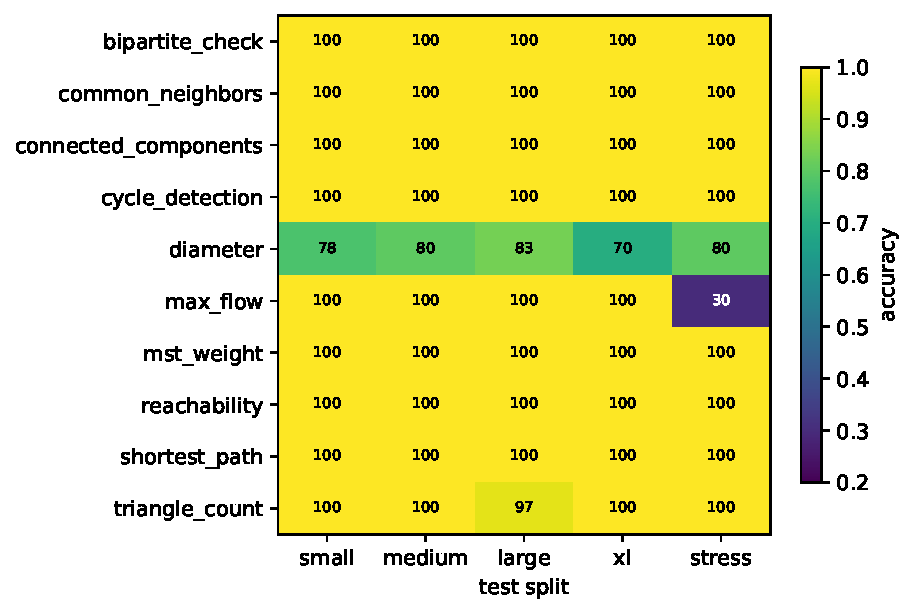
\includegraphics[width=0.86\linewidth]{figures/hda/fig_hda_given_all.pdf}
\caption{Phase-1 test accuracy by task and split.}
\label{fig:p1}
\end{figure}

\subsection{Phase 2: NP-hard tasks}
On exact small references, max clique reaches mean quality 0.931 with 70\%
optimal solutions and 100\% feasibility; MIS reaches 0.971 and 70\% optimal;
MVC reaches only 0.490, is feasible on every instance but never optimal, and
does not improve across iterations (Table~\ref{tab:p2small}). For MVC the model
returns valid but large covers, so the feasibility gate is doing real work.

At larger sizes (Table~\ref{tab:p2large}, Figure~\ref{fig:p2}), max clique
matches the frozen best-known value on every split; this is encouraging but
partly reflects weak large references (best-known sizes 2--11 on sparse
graphs). MIS is the clearest scale signal: quality drops from 0.713 on small
to 0.750 at 500--1000, then 0.153 at 2{,}000 and 0.046 at 10k--20k, and one xl
answer is infeasible. MVC is feasible on 10\% of small graphs and 0\% above
that, so its phase-2 score is effectively zero at scale.

\begin{table}[H]
\centering
\small
\resizebox{\linewidth}{!}{\begin{tabular}{lrrrr}
\toprule
task & val & test q & feasible & optimal \\
\midrule
max\_clique & 94.4\% & 93.1\% & 100\% & 70\% \\
max\_independent\_set & 96.5\% & 97.1\% & 100\% & 70\% \\
min\_vertex\_cover & 45.5\% & 49.0\% & 100\% & 0\% \\
\bottomrule
\end{tabular}
}
\caption{Phase-2 exact small-graph results (3 iterations, $k=5$).}
\label{tab:p2small}
\end{table}

\begin{table}[H]
\centering
\small
\begin{tabular}{lrrrrr}
\toprule
task & small & medium & large & xl & stress \\
\midrule
max\_clique & 95 (100) & 100 (100) & 100 (100) & 100 (100) & 100 (100) \\
max\_independent\_set & 71 (100) & 77 (100) & 75 (100) & 15 (40) & 5 (100) \\
min\_vertex\_cover & 9 (10) & 0 (0) & 0 (0) & 0 (0) & 0 (0) \\
\bottomrule
\end{tabular}

\caption{Phase-2 large results: mean quality (feasible rate in parentheses).
Above 60 nodes the reference is a frozen heuristic, not a proof.}
\label{tab:p2large}
\end{table}

\begin{figure}[H]
\centering
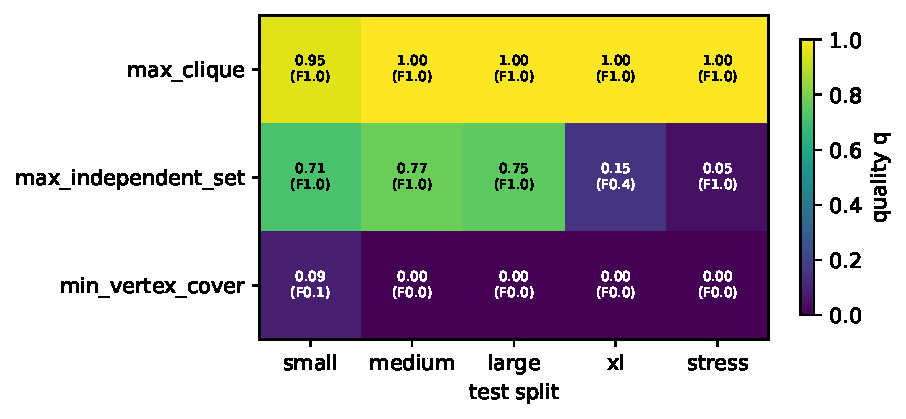
\includegraphics[width=\linewidth]{figures/hda/fig_hda_phase2.pdf}
\caption{Phase-2 quality by task and split; F is the feasible rate.}
\label{fig:p2}
\end{figure}

\section{Discussion and limitations}
The main phase-1 result is that a 4B model can write a correct, scale-safe C++
graph harness for most polynomial tasks when the interface is unambiguous and
the compiler loop is available. The failures are informative: diameter and
max flow are correct on small graphs but weak at the largest sizes, and
triangle counting is nearly perfect. The maximum-flow failure is the cleanest
small-to-large signal.

Phase 2 required a different scoring philosophy. Exact-match scoring would
reject a valid clique with a different node set; normalized quality accepts any
feasible optimum and gives partial credit. MVC shows why the feasibility gate
matters: without it, a large cover would look like a wrong answer; with it, the
program is valid but scores 0.49 and then 0.0 above small graphs.

Limitations: only Qwen3-4B Q4 on CPU was run; the intended gpt-oss-120b/BF16
grid was blocked by the GPU queue. Phase 2 uses one seed and one iteration at
large sizes; best-known references above 60 nodes are heuristics, so
max-clique $q=1$ is not proof of optimality. Hidden-statement runs at scale and
NP-hard integer-programming references are future work. All HDA prose in the
course report is an AI draft and must be rewritten by the authors.

\section*{Supplementary material}
\appendix
\section{Prompt and message structures}
The five message types are shown verbatim below. A is the per-iteration prompt;
B and E are returned after tool steps; C is inserted at the next iteration; D
is returned immediately for an invalid submission.

\lstinputlisting{figures/hda/msg_A.txt}
\lstinputlisting{figures/hda/msg_B.txt}
\lstinputlisting{figures/hda/msg_C.txt}
\lstinputlisting{figures/hda/msg_D.txt}
\lstinputlisting{figures/hda/msg_E.txt}

\section{Tasks and splits}
\begin{table}[H]
\centering
\small
\begin{tabular}{llllp{6.2cm}}
\toprule
task & directed & weighted & query args & statement \\
\midrule
shortest\_path & no & yes & 2 (s,t) & Given an undirected graph with positive integer edge weights and two nodes s and t (the query 2 s t), print the total weight of a minimum-weight path from s to t, or -1 if t is unreachable from s. \\
reachability & yes & no & 2 (s,t) & Given a directed graph and two nodes s and t (query 2 s t), print YES if there is a directed path from s to t, otherwise NO. \\
connected\_components & no & no & none & Given an undirected graph, print the number of connected components (an isolated node is its own component). \\
cycle\_detection & no & no & none & Given an undirected simple graph, print YES if it contains at least one cycle, otherwise NO. \\
diameter & no & no & none & Given a connected undirected unweighted graph, print its diameter: the largest shortest-path distance (in edges) between any two nodes. \\
common\_neighbors & no & no & 2 (s,t) & Given an undirected graph and two nodes u and v (query 2 u v), print the number of nodes adjacent to both u and v. \\
triangle\_count & no & no & none & Given an undirected simple graph, print the number of triangles (unordered triples of mutually adjacent nodes). \\
bipartite\_check & no & no & none & Given an undirected graph, print YES if its nodes can be split into two sets so that every edge joins the two sets (the graph is bipartite), otherwise NO. \\
mst\_weight & no & yes & none & Given a connected undirected graph with positive integer edge weights, print the total weight of a minimum spanning tree. \\
max\_flow & yes & yes & 2 (s,t) & Given a directed graph whose edge weights are capacities and two nodes s and t (query 2 s t), print the value of a maximum flow from s to t. \\
\bottomrule
\end{tabular}

\caption{Phase-1 tasks.}
\end{table}

\begin{table}[H]
\centering
\small
\begin{tabular}{llrrlr}
\toprule
split & nodes & n/task & fam. & limit (s) \\
\midrule
examples & 4-50 & 120 & seen & 1 \\
val & 4-50 & 40 & seen & 1 \\
test\_small & 4-50 & 40 & all & 1 \\
test\_medium & 100-300 & 30 & all & 2 \\
test\_large & 500-1000 & 30 & all & 2 \\
test\_xl & 2000-2000 & 20 & all & 3 \\
test\_stress & 10000-100000 & 10 & all & 5 \\
\bottomrule
\end{tabular}

\caption{Phase-1 splits.}
\end{table}

\begin{table}[H]
\centering
\small
\begin{tabular}{lrrrr}
\toprule
task & small & medium & large & xl/stress \\
\midrule
max clique & 20 & 10 & 8 & 5 / 3 \\
MIS & 20 & 10 & 8 & 5 / 3 \\
MVC & 20 & 10 & 8 & 5 / 3 \\
\bottomrule
\end{tabular}
\caption{Phase-2 test instances per task. Examples/validation remain 60/20
per task at 4--50 nodes.}
\end{table}

\section{Identifiability}
\begin{table}[H]
\centering
\small
\begin{tabular}{lrrrrrp{4.5cm}}
\toprule
task & candidates & k=1 & k=3 & k=5 & k=10 & top confusers at k=3 \\
\midrule
shortest\_path & 4 & 0.81 & 0.98 & 1.00 & 1.00 & edge\_weight, max\_edge\_on\_path \\
reachability & 5 & 0.00 & 0.18 & 0.45 & 0.86 & strongly\_connected, edge\_exists, undirected\_connected \\
connected\_components & 18 & 0.76 & 1.00 & 1.00 & 1.00 & radius\_lcc \\
cycle\_detection & 18 & 0.01 & 0.41 & 0.67 & 0.93 & has\_triangle, is\_connected, is\_tree \\
diameter & 18 & 0.78 & 1.00 & 1.00 & 1.00 & -- \\
common\_neighbors & 7 & 0.60 & 0.97 & 1.00 & 1.00 & min\_degree\_uv, degree\_v, degree\_u \\
triangle\_count & 18 & 0.43 & 0.90 & 0.97 & 1.00 & cycle\_rank, isolated\_nodes \\
bipartite\_check & 18 & 0.23 & 0.74 & 0.92 & 1.00 & is\_connected, is\_tree, cycle\_detection \\
mst\_weight & 6 & 0.58 & 0.93 & 0.98 & 1.00 & max\_spanning\_tree, total\_weight \\
max\_flow & 7 & 0.16 & 0.54 & 0.77 & 0.98 & min\_out\_in, widest\_path, out\_capacity\_s \\
\bottomrule
\end{tabular}

\caption{Probability that the true task is the unique survivor among 10 tasks
and 37 distractors (400 trials).}
\end{table}

\section{Iteration curves and cost}
\begin{table}[H]
\centering
\small
\begin{tabular}{lrrr}
\toprule
task & val curve & test q & tokens (prompt/completion) \\
\midrule
max clique & .944/.755/.944 & .931 & 69k / 6.1k \\
MIS & .664/.965/.965 & .971 & 97k / 8.7k \\
MVC & .455/.455/.455 & .490 & 72k / 6.0k \\
\bottomrule
\end{tabular}
\caption{Phase-2 small-grid curves and token cost.}
\end{table}

\section{Implementation, logging and reproduction}
The pipeline is in \texttt{hda\_pipeline/}. Each run writes \texttt{log.jsonl}
with the config, examples, full prompt, raw reply/reasoning, action, statement,
code, tool results, submissions with per-graph answers and verdicts, iteration
summaries and test rows; \texttt{final.json} holds the validation curve,
statements, tokens and test summaries. Large artifacts stay out of git.
Commands:
\begin{verbatim}
python -m pytest -q tests
python -m hda.generator --out data/hda
python -m hda.generate_phase2 --out data/hda_phase2
python -m hda.agent --task max_clique --condition given \
  --k 5 --n-iter 3 --steps 8 --data data/hda_phase2 \
  --out runs/max_clique --base-url http://HOST:PORT/v1
python -m hda.aggregate --runs runs/main --out report/tables/hda
\end{verbatim}

\begin{thebibliography}{9}
\bibitem{grapharena} GraphArena: A benchmark for graph reasoning.
\bibitem{graphqa} GraphQA: A benchmark for graph question answering.
\bibitem{gepa} GEPA: reflective prompt evolution.
\bibitem{skillopt} SkillOpt: skill-level optimization.
\bibitem{rrsi} RRSI: regularized reflective self-improvement.
\bibitem{evoskill} EvoSkill: evolving reusable skills.
\end{thebibliography}

\end{document}
